\documentclass{beamer}
\mode<presentation>

\usepackage{mathrsfs}   % For scripted math letters
%\usepackage{fixpauseincludegraphics}
\setbeamercovered{dynamic} % for pausing images
\usepackage[english]{babel}
\usepackage[utf8x]{inputenc}
\usepackage{amsmath}
\usefonttheme{serif}
\usetheme{Boadilla}
\usepackage{listings}
\usepackage{color,soul}
\lstset{language=R}
\newcommand{\Mod}[1]{\ (\text{mod}\ #1)}
\newcommand\floor[1]{\lfloor#1\rfloor}
\newcommand\ceil[1]{\lceil#1\rceil}
\newcommand{\lenitem}[2][.7\linewidth]{\parbox[t]{#1}{\strut #2\strut}}
	
\title{Advanced Supervised learning in \\ 
	multi-layer perceptrons \\-  From backpropagation to adaptive learning algorithm}
\author{Venkatramani Rajgopal}
\institute[] 
{\	Department of Mathematics\\
		University of Applied Sciences, Mittweida}
	

\date{14 December 2016} 
\subject{}
\begin{document}

\begin{frame}
\titlepage
\end{frame}

\begin{frame}{Outline}
\tableofcontents
% You might wish to add the option [pausesections]
\end{frame}	


\section{Introduction}
\begin{frame}{Introduction}
\begin{itemize}
\item Discuss the concept of supervised learning in multi layer perceptrons based on gradient descent technique.  	
\item We introduce \textit{Backpropagation} which is one of the most popular training algorithms for multilayer perceptrons. 
\item Some problems and drawbacks of backpropagation learning procedure. 
\item Over the last years many improvement strategies have been developed to speed up backpropagation. We look at some of many different speedup techniques. 


\end{itemize}	

	
\end{frame}	


\section{Preliminaries}
\subsection{Multi Layer Perceptrons}
\begin{frame}{Preliminaries}{Multi Layer Perceptrons}
Multi layer perceptron (Werbos 1974, Rumelhart, McClelland, Hinton 1986), is a \textit{feed-forward network}, consisting of neurons connected by weighted links. 

It is a finite acyclic graph. The nodes are neurons with \textcolor{blue}{sigmoid activation}.

\begin{figure}
\centering
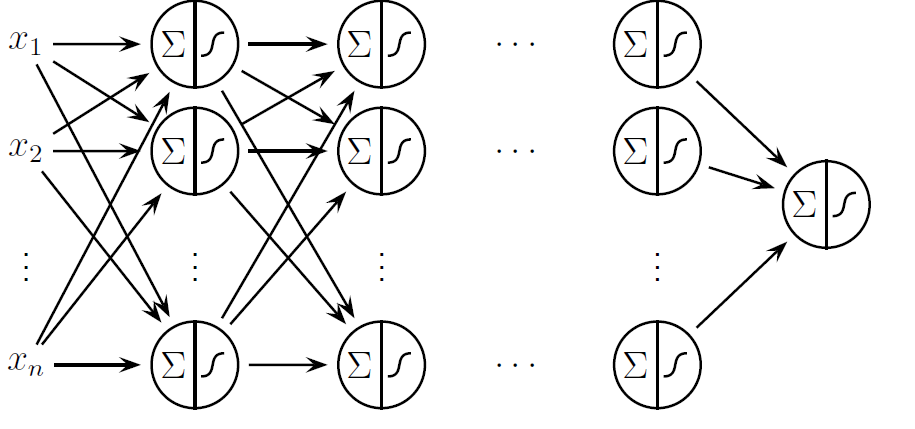
\includegraphics[width=0.5\linewidth]{mlp}
\end{figure}

Units are organised namely, an input layer, hidden layer/s and an output layer. 

\end{frame}

\begin{frame}{Preliminaries}{Multi Layer Perceptrons}
\begin{itemize}
\item Nodes that are no target of any connection are called \textcolor{blue}{input neurons}. A MLP that should be applied to input patterns of dimension n must have n input neurons, one for each dimension. 
\item Nodes that are no source of any connection are called \textcolor{blue}{output neurons}. A
MLP can have more than one output neuron. The number of output neurons depends on the way the target values (desired values) of the training patterns are described. 
\item All nodes that are neither input neurons nor output neurons are called \textcolor{blue}{hidden neurons}

\end{itemize}
\end{frame}	

\begin{frame}{Preliminaries}{Multi Layer Perceptrons}
Variables for calculation. 
\vspace{5mm}
\begin{itemize}
\item \textit{Succ(i)} and \textit{Pred(i)} is the set of all neurons $ j $ for which connection $ i \rightarrow j $ and $ j \rightarrow i $ exists respectively.  
\item The weight of the connection $ j \rightarrow i $ is $ w_{ij} $. 
\item All hidden and output neurons have a bias weight named as $ \theta_i $ for neuron $ i $.  
\item Hidden and output neurons have some variable $ \text{\textit{net}}_{i} $  (network input)and $ s_i $ as its (activation/output). 
\end{itemize}	

\end{frame}	

\begin{frame}{Preliminaries}{Multi Layer Perceptrons}
Applying $ \vec{x} $ to the MLP, 

\begin{itemize}
\item for each input neuron the respective element of the input pattern is presented as, $ s_i \leftarrow x_i $. 
\item for all hidden and output neurons $ i $, calculate  $ \text{\textit{net}}_{i} $ and $ s_i $ as : \\
$  \text{\textit{net}}_{i} = \sum_{j \in \textit{pred(i)}}  s_j w_{ij} - \theta_i$

\pause
\item The activation of unit $ i $, $ s_i $ is computed by passing the net input through a non-linear activation function, usually \textcolor{blue}{sigmoid logistic function.}
\begin{equation*}
s_i = f_{log}(net_i) = \frac{1}{1+ e^{-net_i}}
\end{equation*}

\item A nice property of this function is its easily computable derivative. 
\begin{equation*}
\frac{\partial s_i}{\partial net_i} = f'_{log}(net_i) = s_i * (1-s_i)
\end{equation*}

\end{itemize}
	
\end{frame}	


\subsection{Supervised Learning}
\begin{frame}{Preliminaries}{Supervised Learning}
\textcolor{blue}{Objective:} To tune the weights in the network such that the network performs a desired mapping of input to output activations. 

\pause
\begin{itemize}
\item The mapping is given by a set, the so called pattern set $ \mathscr{P} $. 
\item Each pattern pair $ p $, consist of an input activation vector $ x^p $ and target activation vector $ t^p $. 
\item After training the weights, when an input activation $ x^p $ is presented, the resulting output vector $ s^p $ should equal the target $ t^p $. 
\pause
\item The distance between the target and the actual output vector, is measured by the following cost function $ E: $. 
\begin{equation*}
	E := \frac{1}{2} \sum_{p \in \mathscr{P}} \sum_{n} (t_n^{p} - s_n^{p})^2
\end{equation*}
\end{itemize}	
\end{frame}


\begin{frame}{Preliminaries}{Supervised Learning}
Learning means: calculating weights for which the error $ E $ becomes minimal. \\ 

\vspace{3mm}
The weights in the network are changed along a \textit{search direction }$ d(t) $,
\begin{equation*}
\Delta w(t) = \epsilon * d(t)
\end{equation*}
where the \textcolor{blue}{learning rate} $ \epsilon $, scales the size of the weight step. \\ 

\vspace{3mm}
To determine the search direction $ d(t) $, we use the first order derivative, the \textcolor{blue}{gradient}  
\[ \Delta E = \frac{ \partial E }{\partial w} \]  
\end{frame}


\subsection{Back Propagation algorithm}
\begin{frame}{Preliminaries}{Back Propagation algorithm}
The Back propagation algorithm, performs successive computations of $ \Delta E $, by propagating the error back from output towards the input layer.   	\\

\pause
Idea: Compute the partial derivative $ \partial E / \partial w_{ij} $ for each weight in the network, by repeatedly applying the chain rule: 

\begin{equation*}
\frac{\partial E}{\partial w_{ij}} = \frac{\partial E}{\partial s_{i}} \frac{\partial s_i}{\partial w_{ij}}
\end{equation*}
where,

\begin{equation*}
\frac{\partial s_i}{\partial w_{ij}} = \frac{\partial s_i}{\partial{net_{i}}} \frac{\partial {net_i}}{\partial w_{ij}} = f'_{log} (net_i) s_j
\end{equation*}	


\end{frame}

\begin{frame}{Preliminaries}{Back Propagation algorithm}
To compute $ \partial E / \partial s_i $, we look at the two cases:

\pause
\begin{itemize}
\item If $ i $ is an output unit then, 
\begin{equation*}
\frac{\partial E}{\partial s_{i}}  = \frac{1}{2} \frac{\partial (t_{i} - s_{i})^2}{\partial s_{i}} = -(t_i - s_i)
\end{equation*}

\pause
\item If $ i $ is not an output unit, then we apply the chain rule again;

\begin{align*}
\frac{\partial E}{\partial s_{i}}  & = \sum_{k \in succ(i)} \frac{\partial E}{\partial s_{k}} \frac{\partial s_{k}}{\partial s_{i}} \\
 & = \sum_{k \in succ(i)} \frac{\partial E}{\partial s_{k}}  \frac{\partial s_k}{\partial {net_{k}}}  \frac{\partial {net_k}}{\partial s_{i}} \\
 &= \sum_{k \in succ(i)} \frac{\partial E}{\partial s_{k}} f'_{log} (net_k) w_{ki}
\end{align*}

\end{itemize} 
\end{frame}


\subsection{Gradient Descent}
\begin{frame}{Preliminaries}{Gradient Descent}
The next step in backpropagation is to compute the \textcolor{blue}{weight update}. 	 

\pause
\begin{itemize}
\item Weight update is a scaled step in the opposite direction of the gradient. 
\item The negative derivative is multiplied by a constant value, the \textcolor{blue}{learning-rate}, $ \epsilon $. 
\item We call this minimization technique as \textcolor{blue}{gradient descent}:
\begin{equation*}
\Delta w_{ij} (t) = - \epsilon * \frac{\partial E}{\partial w_{ij} } (t)
\end{equation*} 	
\end{itemize}		

\end{frame}

\begin{frame}{Preliminaries}{Gradient Descent}
Choosing the learning rate. \\

A good choice depends on the error-function. 
\begin{figure}
	\includegraphics<1>[scale=0.5]{gd1}
	\includegraphics<2>[scale=0.5]{gd2}
	\includegraphics<3>[scale=0.5]{gd3}
	\includegraphics<4>[scale=0.5]{gd4}
	\includegraphics<5>[scale=0.5]{gd5}		
	%\caption{\only<1>{Hallo}\only<2>{Welt}}
\end{figure}
	
\end{frame}	

\begin{frame}{Preliminaries}{Gradient Descent - Problems}
\begin{itemize}
\item The weight step is dependent on both the learning parameter and the size of the partial derivative $ \partial E / \partial w_{ij} $. 	

\pause
\item \textcolor{blue}{Flat spots and steep valleys:} \\
We need larger $ \epsilon $ in $ \vec{u} $ to jump over the flat area but need smaller $ \epsilon $ in $ \vec{v} $ to meet the minimum. 


\begin{figure}
\centering
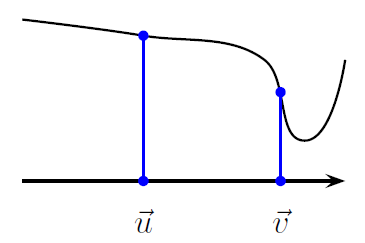
\includegraphics[width=0.3\linewidth]{gdproblem}
\end{figure}

\item \textcolor{blue}{Zig-zagging}
In higher dimensions: $ \epsilon $ is not appropriate for all dimensions. 


\begin{figure}
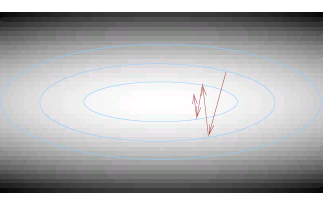
\includegraphics[width=0.3\linewidth]{zig}
\end{figure}

\end{itemize}
\end{frame}

\begin{frame}{Preliminaries}{Gradient Descent - Problems}
Finding the right $ \epsilon $ is annoying. Approaching the minimum is time consuming.

\vspace{5mm}
Heuristics to overcome problems of gradient descent:

\begin{itemize}
\item Gradient descent with momentum
\item Individual learning rates for each dimension
\item Adaptive learning rates
%\item decoupling steplength from partial derivates
\end{itemize}

\end{frame}

\begin{frame}{Preliminaries}{Gradient Descent with momentum}
To make learning more stable, one of the idea was to introduce a \textcolor{blue}{momentum term}, $ \mu $ : 

\pause
\begin{equation*}
\Delta w_{ij} = - \epsilon \frac{\partial E}{\partial w_{ij}} (t) + \mu \Delta w_{ij} (t-1) 
\end{equation*}

It scales the influence of previous weight step on the current one. 	\\

\vspace{4mm}	
	Usually, when using gradient descent with momentum, the learning rate should be decreased to avoid unstable learning. 
\end{frame}

\begin{frame}{Preliminaries}{Gradient Descent with momentum}
Advantages of momentum 
\vspace{8mm}
\begin{itemize}
\item Smoothes zig-zagging
\item Accelerates learning at flat spots
\item Slows down when signs of partial derivatives change
\end{itemize}

\end{frame}

\subsection{Learning by pattern vs learning by epoch}	
\begin{frame}{Preliminaries}{Learning by pattern vs learning by epoch}
Two methods for computing weight update. \\
\vspace{5mm}

\begin{itemize}
\item In \textcolor{blue}{learning by pattern} method a weight update is performed after computation of respective gradient. This is known as \textcolor{blue}{online learning.}

\item \textcolor{blue}{Learning by epoch} first sums the gradient information for the whole pattern set, then performs the weight update. Known as \textcolor{blue}{batch learning}.  
\end{itemize}

\end{frame}


\section{Global Adaptive Techniques}	
\subsection{Steepest descent}
\begin{frame}{Global Adaptive Techniques}{Steepest Descent}
Adaptive learning rate. 
\vspace{5mm}
\pause
Idea: 
\begin{itemize}
\item Make learning rate individual for each dimension and adaptive
\item If signs of partial derivative change, reduce learning rate
\item If signs of partial derivative don’t change, increase learning rate
\end{itemize}
\vspace{5mm}

Algorithms, that use the global knowledge of the entire network, like \textit{direction} of the overall weight update are referred as \textcolor{blue}{global} techniques.  

\end{frame}


\begin{frame}{Global Adaptive Techniques}{Steepest Descent}
The steepest descent tries to take an \textcolor{blue}{optimal weight step} by finding an \textcolor{blue}{individual scaling parameter $ \epsilon(t) $}, each iteration. 

\begin{itemize}
\item To find such a parameter, is regarded as \textcolor{blue}{line search.}
\item A small initial learning rate is used, which is increased until the error function no longer decreases. 
\end{itemize}
\pause
\vspace{5mm}
\textcolor{red}{Drawback}: For every iteration, the evaluation of the error function $ E $ is required, which is a costly propagation, to compute the new value of $ E $.  

\end{frame}

\begin{frame}{Global Adaptive Techniques}{Steepest Descent}
While applying Steepest Descent, it can be shown that two successive weight steps are perpendicular. 	
	
	
\begin{equation*}
\frac{\partial(w(t+1))}{\partial\epsilon} = 0 
\end{equation*}

Then, 
\begin{align}
\label{SD}
\frac{\partial(w(t+1))}{\partial \epsilon}  & = \frac{\partial(w(t+1))}{\partial w(t+1)} \frac{\partial (w(t) + \epsilon * \partial(t))}{\partial \epsilon} \nonumber \\ 	
& = \nabla E(t+1) d(t) \nonumber \\
& = 0
\end{align} 

Means that the new gradient $ \nabla E(t+1) $ that determines the new direction $ d(t+1) $ and old direction $ d(t) $ are perpendicular.  

\end{frame}

\subsection{Conjugate gradient method}
\begin{frame}{Global Adaptive Techniques}{Conjugate gradient method}
\begin{figure}
\centering
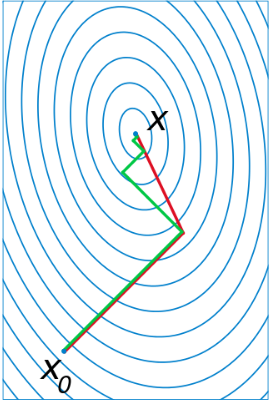
\includegraphics[width=0.25\linewidth]{conjugategrad}
\end{figure}
Comparison of the convergence of gradient descent with optimal step (in green) and conjugate vector (in red). 

\end{frame}
	

\begin{frame}{Global Adaptive Techniques}{Conjugate gradient method}

The condition from Equation (\ref{SD}) also holds good for the weight step, 
\begin{equation*}
d(t) \nabla E(t+2) = 0
\end{equation*}

and it can be shown that above is fulfilled if, 

\begin{equation}
\label{Hessian}
d(t) \mathscr{H} d(t+1) = 0 
\end{equation}

where $ \mathscr{H} $ denotes that Hessian Matrix, containing second order derivatives of the weights. 
\vspace{3mm}
Two vectors fulfilling the above are called \textcolor{blue}{conjugate}. 


\end{frame}

\begin{frame}{Global Adaptive Techniques}{Conjugate gradient method}
To determine the new search direction $ d(t+1) $ that fulfills equation (\ref{Hessian}) we set,
\begin{equation*}
d(t+1) = - \nabla E(t+1) + \beta * d(t)
\end{equation*}
\pause
This means that the new search direction is a combination of the direction indicated by the gradient and the previous search direction. \\

\vspace{5mm}
The parameter $ \beta $ is computed using the Polak-Ribiere rule:

\begin{equation*}
\beta = \frac{(\nabla E(t+1)  - \nabla E(t)) \nabla E(t+1)}{(\nabla E(t))^2}	
\end{equation*}
	
\end{frame}	
	
	
\section{Local adaptive techniques}
\subsection{Delta bar delta rule}
\begin{frame}{Local adaptive techniques}{Delta bar delta rule}
R Jacobs, proposed the 	\textcolor{blue}{weight specific learning rates}. He determined the evolution of learning rates according to the estimation of the shape of the error function. 

\pause
\begin{itemize}
\item Based on the observed behaviour of the partial derivatives during two successive weight steps. 
\item If derivatives have same sign, the learning rate is linearly increased by a small constant.  
\item On the other hand, a change in sign of the two derivatives indicates that the procedure has over shot a local minimum. (i.e the the previous weight step was too large). 
\item As a consequence, the learning rate is decreased. 
\end{itemize}
\end{frame}	

\begin{frame}{Local adaptive techniques}{Delta bar delta rule}
Which is,	

\[
\epsilon_{ij}^{(t)} = \begin{cases}
	\kappa + \epsilon_{ij}^{(t-1)} , & \text{if} \qquad \frac{\partial E^{(t-1)}}{\partial w_{ij}} * \frac{\partial E^{(t)}}{\partial w_{ij}} > 0 \\
	
	\eta^- * \epsilon_{ij}^{(t-1)} , & \text{if} \qquad \frac{\partial E^{(t-1)}}{\partial w_{ij}} * \frac{\partial E^{(t)}}{\partial w_{ij}} < 0 \\
	
	\epsilon_{ij}^{(t-1)} , & \text{else}

\end{cases}
\]

with $  0< \eta^- < 1 $. \\
\pause
\vspace{3mm}
\textcolor{blue}{Weight update} is the same as with backpropagation learning, except that, the fixed learning rate $ \epsilon $ is replaced by the weight specific, dynamic learning rate $ \epsilon_{ij} (t) $

\begin{equation*}
\Delta w_{ij} (t)  = -\epsilon_{ij}(t) \frac{\partial E}{\partial w_{ij}}(t) + \mu \Delta w_{ij} (t-1) 
\end{equation*}

\end{frame}

\subsection{SuperSAB}
\begin{frame}{Local adaptive techniques}{SuperSAB}
	\begin{itemize}
\item Based on the idea of \textcolor{blue}{sign-dependent learning rate adoption}. \\

\item Change here, is to increase the learning rate \textcolor{blue}{exponentially } instead of linearly like in Delta Bar Delta rule. 

\pause
\[
\epsilon_{ij}^{(t)} = \begin{cases}
\eta^+ + \epsilon_{ij}^{(t-1)} & ,  \text{if} \qquad \frac{\partial E^{(t-1)}}{\partial w_{ij}} * \frac{\partial E^{(t)}}{\partial w_{ij}} > 0 \\

\eta^- * \epsilon_{ij}^{(t-1)} & ,  \text{if} \qquad \frac{\partial E^{(t-1)}}{\partial w_{ij}} * \frac{\partial E^{(t)}}{\partial w_{ij}} < 0 \\

\epsilon_{ij}^{(t-1)} & ,  \text{else}

\end{cases}
\]

with $  0< \eta^- < 1 < \eta^+ $. 		
	\end{itemize}
Also, in case of a change in sign of two successive derivatives, the previous weight step is reverted.

\end{frame}	

\begin{frame}{Local adaptive techniques}{SuperSAB}
Advantage:\\
Fast convergence. Often faster than ordinary gradient descent. 
\vspace{4mm}

\textcolor{red}{Disadvantage}:\\
Determination of large number of parameters to achieve good convergence. \\
Initial learning rate, the momentum factor 	and the increase (decrease) factor. 
	
\begin{equation*}
\Delta w_{ij} (t)  = -\epsilon_{ij}(t) \frac{\partial E}{\partial w_{ij}}(t) + \mu \Delta w_{ij} (t-1) 
\end{equation*}	
	
\end{frame}	

\subsection{Quickprop Algorithm}
\begin{frame}{Local adaptive techniques}{Quickprop}
Local adaptive techniques are based on weight specific information, such as the behaviour of the partial derivative. 	
\vspace{3mm}

\textcolor{blue}{Idea}: To find a solution in a short time, taking the largest step possible, without overshooting the solution. 
	
	\pause
	
\begin{itemize}


\item Here we make explicit use of the second derivative of the error with respect to each weight. \\


\item It is a second-order method, based loosely on \textcolor{blue}{Newton’s method}. \\ 
\item Everything proceeds as in standard back-propagation, but for each weight, keep a copy of $ \partial E / \partial w(t-1) $, the error derivative computed during the previous training epoch, along with the difference between the current and previous values of this weight. 

\end{itemize}	

\end{frame}

\begin{frame}{Quickprop}
\begin{block}{Assumption}
Local error function for each weight is assumed to be a 'Parabalo whose arms are wide open'. \\
%Slope of the curve is not effected by changing all other weights in the network. 
\end{block}

\pause
For each weight, independently, we use the previous and current error slopes and the weight-change between the points at which these slopes were measured to determine a parabola; we then jump directly to the \textit{minimum point of this parabola}.

\pause
\vspace{4mm}
So the update rule we have; 
\begin{equation}
\label{updaterule}
\Delta w_{ij} (t) = \frac{\frac{\partial E}{\partial w_{ij}} (t) }{\frac{\partial E}{\partial w_{ij}} (t-1) - \frac{\partial E}{\partial w_{ij} (t)}} \Delta w(t-1)
\end{equation}

\end{frame}

\begin{frame}{Quickprop}
\begin{itemize}
\item The update rule is equivalent to Newtons approximation method. 
\item The objective is to find a minimum of $ f(x) $
\item Newtons method computes updates of $ x $ according to ;
\begin{equation*}
x(t+1) = x(t) + \Delta x(t)
\end{equation*}

where,

$ \Delta x(t)  = - \frac{f'(x(t))}{f"(x(t))}$ 

\vspace{2mm}
Approximation using the first order derivatives: 

\begin{align*}
f"(x(t)) &= \frac{f'(x(t)) - f'(x(t-1))}{x(t) - x(t-1)}
		 &= \frac{f'(x(t)) - f'(x(t-1))} {\Delta x(t-1)}	
\end{align*} 
\end{itemize}
\end{frame}	

\begin{frame}{Quickprop}
\begin{itemize}
\item By substitution we have, 
\begin{equation}
\Delta x(t) =  \frac{f'(x(t))} { f'(x(t-1)) -f'x(t)} \Delta x(t-1)  
\end{equation}

which corresponds to the update rule  $ \Delta w_{ij}(t) $. (Equation (\ref{updaterule}))

\item The update rule is composed of $ \Delta w_{ij}(t) $ and a small gradient step. \\ 

\pause
\vspace{4mm}
\item To avoid large weight steps, coming from small denominator, the \textcolor{blue}{present weight step is restricted to at most $ \nu $ times} as large as the previous step. \\

\item The Quickprop thus has two parameters. \\
Learning rate $ \epsilon $ for gradient descent and a second parameter $ \nu  $ which limits the step size. 
	
\end{itemize}	

\end{frame}	

\subsection{Rprop}
\begin{frame}{Rprop - Resilient backpropagation}
The basic idea here is to eliminate the harmful influence of the size of the partial derivative on the weight step. 

\pause
\begin{itemize}
\item To achieve this, we introduce for each weight its \textcolor{blue}{individual update value} $ \Delta_{ij} $, which solely determines the size of the weight update. 

%\textit{First}, it only uses the sign of the gradient, to indicate the direction of the weight update. The size of the weight change is determined by a \textit{weight specific}, \textit{update-value} $ \Delta _{ij} $ :

\[
\Delta_{ij}^{(t)} = \begin{cases}
\eta^+ + \Delta_{ij}^{(t-1)} & ,  \text{if} \qquad \frac{\partial E^{(t-1)}}{\partial w_{ij}} * \frac{\partial E^{(t)}}{\partial w_{ij}} > 0 \\

\eta^- * \Delta_{ij}^{(t-1)} & ,  \text{if} \qquad \frac{\partial E^{(t-1)}}{\partial w_{ij}} * \frac{\partial E^{(t)}}{\partial w_{ij}} < 0 \\

\Delta_{ij}^{(t-1)} & ,  \text{else}

\end{cases}
\]

where $  0< \eta^- < 1 < \eta^+ $.




\end{itemize}
\end{frame}

\begin{frame}{Rprop - Resilient backpropagation}
Adaptation rule:
 
\begin{itemize}
\item Every time the partial derivative of the corresponding weight $ w_{ij} $ changes its sign, which indicates that the last update was too big and the algorithm has jumped over a local minimum, the update-value $ \Delta_{ij} $ is decreased by a factor of $ \eta^- $. 
\item If the derivative retains its sign, the update-value is slightly increased in order to accelerate convergence in shallow regions.  
\end{itemize}

%\textit{Second}, is to determine the new update values $ \Delta_{ij} (t) $, based on the sign dependent adaptation process, similar to \textit{SuperSAB}. 





\end{frame}

\begin{frame}{Rprop - Resilient backpropagation}
Once the update-value for each weight is adapted, the weight-update itself follows a very simple rule: 
\begin{itemize}
\item If the derivative is positive (ie if we have an increasing error), the weight is decreased by its update-value. 
\item If the derivative is negative, the update-value is added.


\[
\Delta w_{ij}^{(t)} = \begin{cases}
- \Delta_{ij}^{(t)} & ,  \text{if} \qquad \frac{\partial E}{\partial w_{ij}}^{(t)} > 0 \\

+ \Delta_{ij}^{(t)} & ,  \text{if} \qquad \frac{\partial E}{\partial w_{ij}}^{(t)} < 0 \\

0 & ,  \text{else}

\end{cases}
\]



\end{itemize}

\end{frame}


\begin{frame}{Rprop - Resilient backpropagation}
\textit{Exception:} If the partial derivative changes sign, i.e. the previous step was too large and the minimum was missed, the previous weight-update is reverted: \\

\[ \Delta w_{ij}^{(t)} = - \Delta w_{ij}^{(t-1)} \text{, if} \qquad \frac{\partial E^{(t-1)}}{\partial w_{ij}} * \frac{\partial E^{(t)}}{\partial w_{ij}} < 0 \]



\end{frame}

\begin{frame}{Rprop - Resilient backpropagation}
Parameters.	

\vspace{5mm}

\begin{itemize}

\item Beginning: all update values $ \Delta_{ij} $ are set to an initial value of $ \Delta_0 $. 

\item The second paramater is the upper bound $ \Delta_{max} $. This is set inorder to prevent the weights from becoming too large, max weight step determined by the size of the update value is limited. 
	
\item The increase and decrease factors are fixed to $ \eta^{+} = 1.2 $ and $ \eta^{-} = 0.5 $. 
	
\end{itemize}
	
\end{frame}

\begin{frame}{Rprop - Resilient backpropagation}
Main advantages of RPROP - For many problems no choice of parameters is needed at all to obtain optimal convergence. \\

\vspace{3mm}
To summarize,
\vspace{3mm}

\begin{itemize}
\item Rprop is the direct adaptation of the weight update values $ \Delta_{ij}. $ 
\item It modifies the size of the weight step directly by introducing a concept of \textit{resilient update-values.} 
\item As a result adaptation effort is not blurred by unforeseeable gradient behaviour. 
\end{itemize}

\end{frame}

\section{Test Results}
\begin{frame}{Test Results}
\begin{figure}
\centering
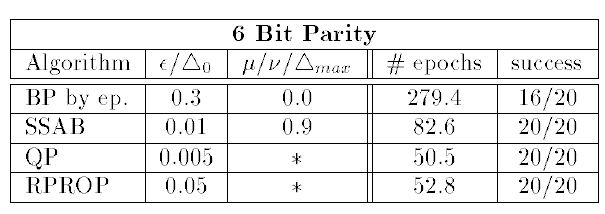
\includegraphics[width=0.45\linewidth]{3bitparity}
\caption{\small{Results for different learning procedures}}
\label{fig:3bitparity}
\end{figure}

\begin{figure}
	\centering
	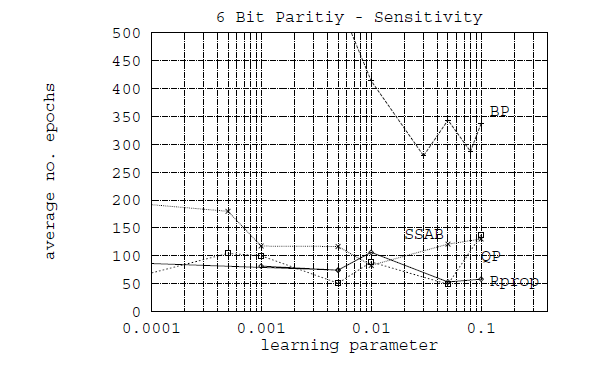
\includegraphics[width=0.5\linewidth]{3bitparity_sensitivity}
	\caption{\small {Sensitivity of different learning procedures to choice of learning parameter}}
	\label{fig:3bitparity}
\end{figure}

\end{frame}



\begin{frame}[allowframebreaks]
	\frametitle<presentation>{References}	
	\begin{thebibliography}{10}
		
		%\beamertemplatearticlebibitems			
		%\bibitem{}
		
		%\newblock {\em }
		
	
		
\beamertemplatearticlebibitems		
		\bibitem{}
		Martin Riedmiller
		\newblock {\em Advanced supervised learning in Multi layer perceptrons. \\ 
			From Back propagation to adaptive learning algorithms}\\
		
		\newblock {Institut für Logik, Komplexitdt und Deduktionssysteme, University of Karlsruhe,Germany }
		
\beamertemplatearticlebibitems	
		\bibitem{}
		Scott E. Fahlman
		\newblock {\em An Empirical Study of Learning Speed in Back-Propagation Networks \\}
		September 1988, CMU-CS-88-162
		
\beamertemplatearticlebibitems	
\bibitem{}
Martin Riedmiller, Heinrich Braun
\newblock {\em A Direct Adaptive Method for Faster Backpropagation Learning: The RPROP Algorithm \\}
\newblock {Institut für Logik, Komplexitdt und Deduktionssysteme, University of Karlsruhe,Germany}

		
		\end{thebibliography}
\end{frame}

%\begin{frame}
%	\centering
%	Thank You for your attention. 
%\end{frame}


\end{document}
